\documentclass[11pt,a4paper]{report}
\usepackage[textwidth=37em,vmargin=30mm]{geometry}
\usepackage{calc,xunicode,amsmath,amssymb,paralist,enumitem,tabu,booktabs,datetime2,xeCJK,xeCJKfntef,listings}
\usepackage{tocloft,fancyhdr,tcolorbox,xcolor,graphicx,eso-pic,xltxtra,xelatexemoji}

\newcommand{\envyear}[0]{2025}
\newcommand{\envdatestr}[0]{2025-01-22}
\newcommand{\envfinaldir}[0]{webdb/2025/20250122/final}

\usepackage[hidelinks]{hyperref}
\hypersetup{
    colorlinks=false,
    pdfpagemode=FullScreen,
    pdftitle={Web Digest - \envdatestr}
}

\setlength{\cftbeforechapskip}{10pt}
\renewcommand{\cftchapfont}{\rmfamily\bfseries\large\raggedright}
\setlength{\cftbeforesecskip}{2pt}
\renewcommand{\cftsecfont}{\sffamily\small\raggedright}

\setdefaultleftmargin{2em}{2em}{1em}{1em}{1em}{1em}

\usepackage{xeCJK,xeCJKfntef}
\xeCJKsetup{PunctStyle=plain,RubberPunctSkip=false,CJKglue=\strut\hskip 0pt plus 0.1em minus 0.05em,CJKecglue=\strut\hskip 0.22em plus 0.2em}
\XeTeXlinebreaklocale "zh"
\XeTeXlinebreakskip = 0pt


\setmainfont{Brygada 1918}
\setromanfont{Brygada 1918}
\setsansfont{IBM Plex Sans}
\setmonofont{JetBrains Mono NL}
\setCJKmainfont{Noto Serif CJK SC}
\setCJKromanfont{Noto Serif CJK SC}
\setCJKsansfont{Noto Sans CJK SC}
\setCJKmonofont{Noto Sans CJK SC}

\setlength{\parindent}{0pt}
\setlength{\parskip}{8pt}
\linespread{1.15}

\lstset{
	basicstyle=\ttfamily\footnotesize,
	numbersep=5pt,
	backgroundcolor=\color{black!5},
	showspaces=false,
	showstringspaces=false,
	showtabs=false,
	tabsize=2,
	captionpos=b,
	breaklines=true,
	breakatwhitespace=true,
	breakautoindent=true,
	linewidth=\textwidth
}






\newcommand{\coverpic}[2]{
    % argv: itemurl, authorname
    Cover photo by #2~~(\href{#1}{#1})
}
\newcommand{\makeheader}[0]{
    \begin{titlepage}
        % \newgeometry{hmargin=15mm,tmargin=21mm,bmargin=12mm}
        \begin{center}
            
            \rmfamily\scshape
            \fontspec{BaskervilleF}
            \fontspec{Old Standard}
            \fontsize{59pt}{70pt}\selectfont
            WEB\hfill DIGEST
            
            \vfill
            % \vskip 30pt
            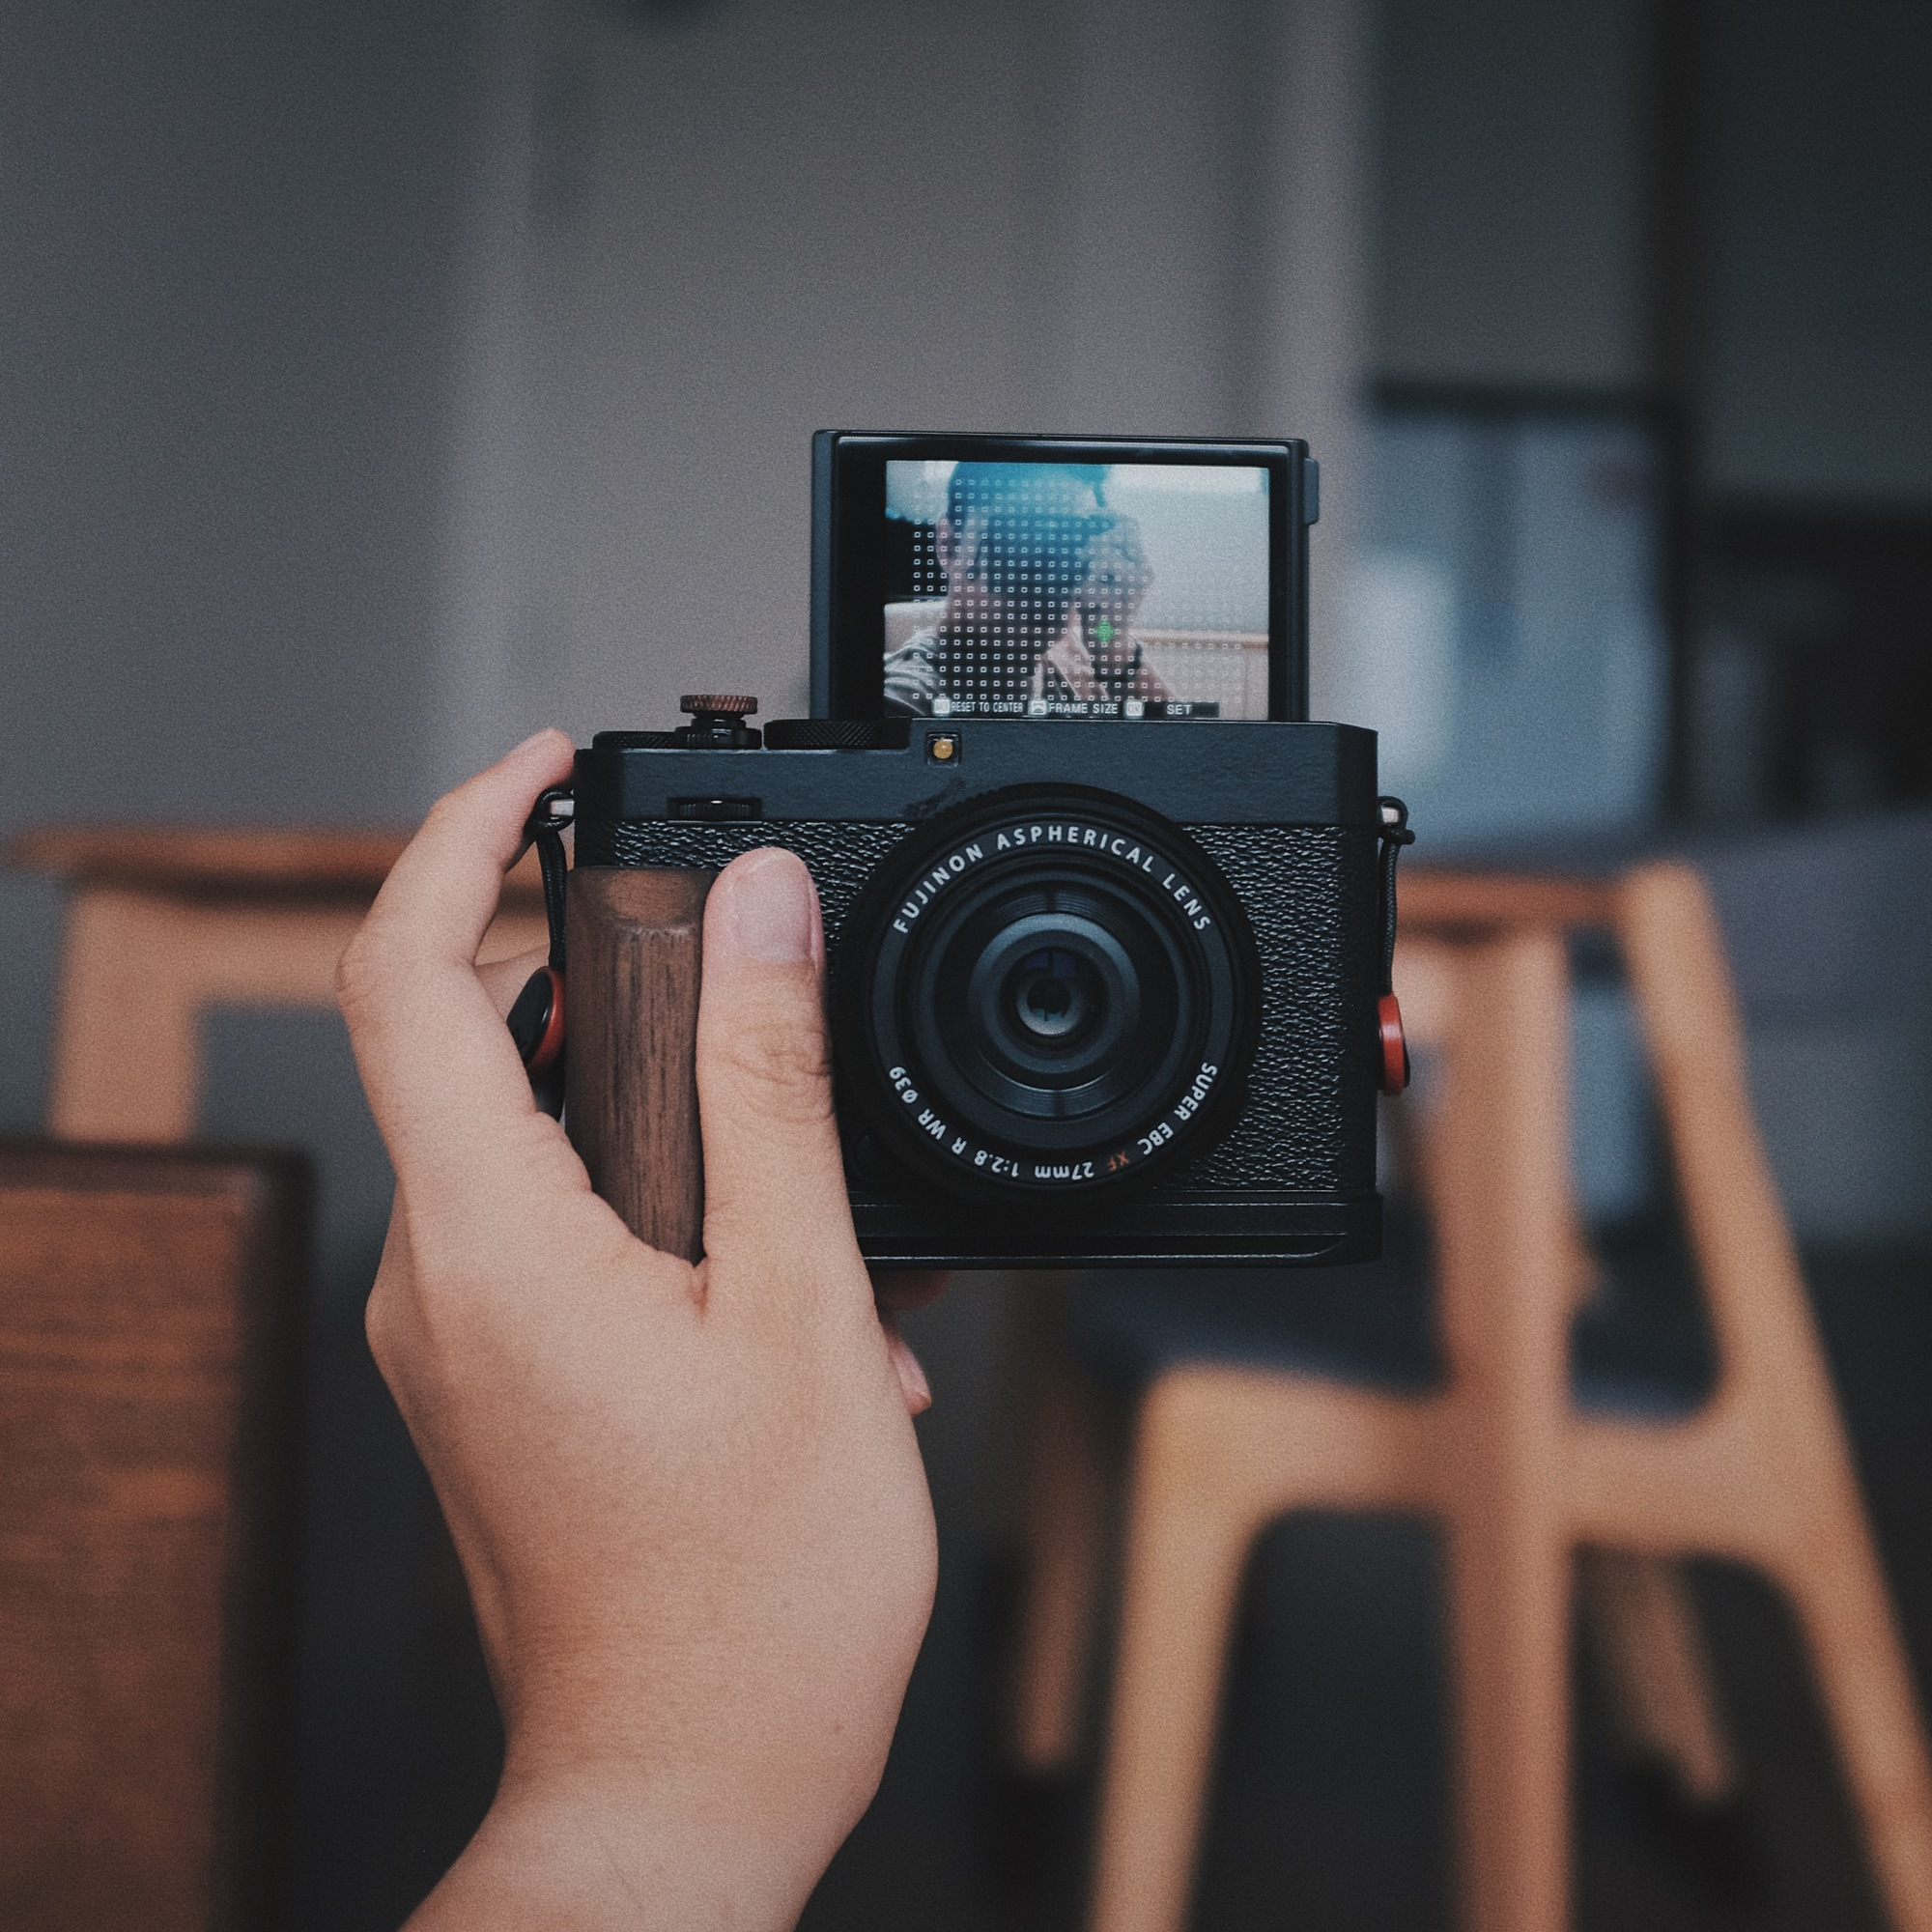
\includegraphics[width=\linewidth]{\envfinaldir/coverpic-prod.jpg}\par
            % \vskip 30pt
            \vfill

            \normalsize\rmfamily\scshape
            \copyright{} The Web Digest Project \hfill\large \envdatestr
        \end{center}
    \end{titlepage}
    % \restoregeometry
}
\newcommand{\simplehref}[1]{%
    \textcolor{blue!80!green}{\href{#1}{#1}}%
}
\renewcommand{\contentsname}{\center\Huge\sffamily\bfseries Contents\par\vskip 20pt}
\newcounter{ipartcounter}
\setcounter{ipartcounter}{0}
\newcommand{\ipart}[1]{
    % \vskip 20pt
    \clearpage
    \stepcounter{ipartcounter}
    \phantomsection
    \addcontentsline{toc}{chapter}{#1}
    % \begin{center}
    %     \Huge
    %     \sffamily\bfseries
    %     #1
    % \end{center}
    % \vskip 20pt plus 7pt
}
\newcounter{ichaptercounter}
\setcounter{ichaptercounter}{0}
\newcommand{\ichapter}[1]{
    % \vskip 20pt
    \clearpage
    \stepcounter{ichaptercounter}
    \phantomsection
    \addcontentsline{toc}{section}{\numberline{\arabic{ichaptercounter}}#1}
    \begin{center}
        \Huge
        \sffamily\bfseries
        #1
    \end{center}
    \vskip 20pt plus 7pt
}
\newcommand{\entrytitlefont}[1]{\subsection*{\raggedright\Large\sffamily\bfseries#1}}
\newcommand{\entryitemGeneric}[2]{
    % argv: title, url
    \parbox{\linewidth}{
        \entrytitlefont{#1}\par\vskip 5pt
        \footnotesize\ttfamily\mdseries
        \simplehref{#2}
    }\vskip 11pt plus 11pt minus 1pt
}
\newcommand{\entryitemGithub}[3]{
    % argv: title, url, desc
    \parbox{\linewidth}{
        \entrytitlefont{#1}\par\vskip 5pt
        \footnotesize\ttfamily\mdseries
        \simplehref{#2}\par\vskip 5pt
        \small\rmfamily\mdseries#3
    }\vskip 11pt plus 11pt minus 1pt
}
\newcommand{\entryitemAp}[3]{
    % argv: title, url, desc
    \parbox{\linewidth}{
        \entrytitlefont{#1}\par\vskip 5pt
        \footnotesize\ttfamily\mdseries
        \simplehref{#2}\par\vskip 5pt
        \small\rmfamily\mdseries#3
    }\vskip 11pt plus 11pt minus 1pt
}
\newcommand{\entryitemHackernews}[3]{
    % argv: title, hnurl, rawurl
    % \parbox{\linewidth}{
    %     \entrytitlefont{#1}\par\vskip 5pt
    %     \footnotesize\ttfamily\mdseries
    %     \simplehref{#3}\par
    %     \textcolor{black!50}{\href{#2}{#2}}
    % }\vskip 11pt plus 11pt minus 1pt
    \begin{minipage}{\linewidth}
            \entrytitlefont{#1}\par\vskip 5pt
            \footnotesize\ttfamily\mdseries
            \simplehref{#3}\par
            \textcolor{black!50}{\href{#2}{#2}}
    \end{minipage}\par\vskip 11pt plus 11pt minus 1pt
}







\begin{document}

\makeheader

\tableofcontents\clearpage




\ipart{Developers}
\ichapter{Hacker News}
\entryitemTwoLinks{Stargate Project: SoftBank, OpenAI, Oracle, MGX to build data centers}{https://news.ycombinator.com/item?id=42785891}{https://apnews.com/article/trump-ai-openai-oracle-softbank-son-altman-ellison-be261f8a8ee07a0623d4170397348c41}

\entryitemTwoLinks{Ask HN: Is anyone doing anything cool with tiny language models?}{https://news.ycombinator.com/item?id=42784365}{https://news.ycombinator.com/item?id=42784365}

\entryitemTwoLinks{Invisible Electrostatic Wall at 3M plant (1996)}{https://news.ycombinator.com/item?id=42782914}{http://amasci.com/weird/unusual/e-wall.html}

\entryitemTwoLinks{Show HN: I made a app that uses NFC as a physical switch to block distractions}{https://news.ycombinator.com/item?id=42782295}{https://www.foqos.app}

\entryitemTwoLinks{Should we use AI and LLMs for Christian apologetics? (2024)}{https://news.ycombinator.com/item?id=42781293}{https://lukeplant.me.uk/blog/posts/should-we-use-llms-for-christian-apologetics/}

\entryitemTwoLinks{Calm tech certification "rewards" less distracting tech}{https://news.ycombinator.com/item?id=42780953}{https://spectrum.ieee.org/calm-tech}

\entryitemTwoLinks{0-click deanonymization attack targeting Signal, Discord, other platforms}{https://news.ycombinator.com/item?id=42780816}{https://gist.github.com/hackermondev/45a3cdfa52246f1d1201c1e8cdef6117}

\entryitemTwoLinks{Metacognitive laziness: Effects of generative AI on learning motivation}{https://news.ycombinator.com/item?id=42780022}{https://bera-journals.onlinelibrary.wiley.com/doi/10.1111/bjet.13544}

\entryitemTwoLinks{Ask HN: Organize local communities without Facebook?}{https://news.ycombinator.com/item?id=42779776}{https://news.ycombinator.com/item?id=42779776}

\entryitemTwoLinks{Couriers mystified by the algorithms that control their jobs}{https://news.ycombinator.com/item?id=42779544}{https://www.theguardian.com/business/2025/jan/21/its-a-nightmare-couriers-mystified-by-the-algorithms-that-control-their-jobs}

\entryitemTwoLinks{People are bad at reporting what they eat. That's a problem for dietary research}{https://news.ycombinator.com/item?id=42779147}{https://www.science.org/content/article/people-are-bad-reporting-what-they-eat-s-problem-dietary-research}

\entryitemTwoLinks{Show HN: Printercow – Turn any thermal printer into an API endpoint}{https://news.ycombinator.com/item?id=42778771}{https://www.printercow.com/}

\entryitemTwoLinks{Startup Winter: Hacker News Lost Its Faith}{https://news.ycombinator.com/item?id=42778266}{https://www.vincentschmalbach.com/startup-winter-hacker-news-lost-its-faith/}

\entryitemTwoLinks{Meta Censoring '\#Democrat' on Instagram}{https://news.ycombinator.com/item?id=42777938}{https://mstdn.chrisalemany.ca/@chris/113864600222476627}

\entryitemTwoLinks{Kimi K1.5: Scaling Reinforcement Learning with LLMs}{https://news.ycombinator.com/item?id=42777857}{https://github.com/MoonshotAI/Kimi-k1.5}

\entryitemTwoLinks{We've lost our respect for complexity}{https://news.ycombinator.com/item?id=42777715}{https://wilsoniumite.com/2025/01/21/weve-lost-our-respect-for-complexity/}

\entryitemTwoLinks{Context should go away for Go 2 (2017)}{https://news.ycombinator.com/item?id=42777625}{https://faiface.github.io/post/context-should-go-away-go2/}

\entryitemTwoLinks{More than 40\% of postdocs leave academia, study reveals}{https://news.ycombinator.com/item?id=42777193}{https://www.nature.com/articles/d41586-025-00142-y}

\entryitemTwoLinks{United States Digital Service Renamed to DOGE}{https://news.ycombinator.com/item?id=42775684}{https://www.whitehouse.gov/presidential-actions/2025/01/establishing-and-implementing-the-presidents-department-of-government-efficiency/}

\entryitemTwoLinks{It sure looks like Meta stole a lot of books to build its AI}{https://news.ycombinator.com/item?id=42775545}{https://lithub.com/it-sure-looks-like-meta-stole-a-lot-of-books-to-build-its-ai/}\ichapter{Phoronix}
\entryitemGeneric{\hskip 0pt{}SDL 3 Officially Released With New APIs, Better HiDPI \& Improved Audio Handling}{https://www.phoronix.com/news/SDL3-Official-Release}

\entryitemGeneric{\hskip 0pt{}Btrfs Changes Land In Linux 6.14 With New RAID1 Round-Robin Option}{https://www.phoronix.com/news/Linux-6.14-Btrfs}

\entryitemGeneric{\hskip 0pt{}New "AMD Node" Driver Introduced In Linux 6.14 For Splitting Up Legacy Northbridge Code}{https://www.phoronix.com/news/Linux-6.14-AMD-NODE}

\entryitemGeneric{\hskip 0pt{}Wine 10.0 Released With Native Wayland Support, Better HiDPI}{https://www.phoronix.com/news/Wine-10.0-Released}

\entryitemGeneric{\hskip 0pt{}Raspberry Pi Monitor Pairs Great With The Raspberry Pi 500 As A \$100 Display}{https://www.phoronix.com/review/raspberry-pi-monitor}

\entryitemGeneric{\hskip 0pt{}Serpent OS Developing disks-rs To Safely Deal With File-Systems \& Block Devices In Rust}{https://www.phoronix.com/news/Serpent-OS-disks-rs}

\entryitemGeneric{\hskip 0pt{}Linux 6.14 Landing Support For FPGA Support On AAEON UP Maker Boards}{https://www.phoronix.com/news/Linux-6.14-AAEON-UP-FPGAs}

\entryitemGeneric{\hskip 0pt{}Linux 6.14 Networking Brings Many Wired \& Wireless Driver Improvements}{https://www.phoronix.com/news/Linux-6.14-Networking}

\entryitemGeneric{\hskip 0pt{}Open-Source Radeon Vulkan Driver "RADV" Seeing More RDNA4 Work In Recent Days}{https://www.phoronix.com/news/RADV-Uptick-In-RDNA4-GFX12}\ichapter{Dribbble}
\entryitemGeneric{\hskip 0pt{}Haptic Logo Design}{https://dribbble.com/shots/25504012-Haptic-Logo-Design}

\entryitemGeneric{\hskip 0pt{}QVELTY / Design \& Animation}{https://dribbble.com/shots/25507639-QVELTY-Design-Animation}

\entryitemGeneric{\hskip 0pt{}Wine Label}{https://dribbble.com/shots/25503830-Wine-Label}

\entryitemGeneric{\hskip 0pt{}Monocle Cat}{https://dribbble.com/shots/25502155-Monocle-Cat}

\entryitemGeneric{\hskip 0pt{}Personal Banking App}{https://dribbble.com/shots/25493958-Personal-Banking-App}

\entryitemGeneric{\hskip 0pt{}404}{https://dribbble.com/shots/25492419-404}

\entryitemGeneric{\hskip 0pt{}Wine Label}{https://dribbble.com/shots/25490604-Wine-Label}

\entryitemGeneric{\hskip 0pt{}planet}{https://dribbble.com/shots/25490310-planet}

\entryitemGeneric{\hskip 0pt{}Shihiko // E-commerce Website}{https://dribbble.com/shots/25489208-Shihiko-E-commerce-Website}

\entryitemGeneric{\hskip 0pt{}Wine Label}{https://dribbble.com/shots/25485370-Wine-Label}

\entryitemGeneric{\hskip 0pt{}Roam Supply Co. - Shirt Graphic}{https://dribbble.com/shots/25433659-Roam-Supply-Co-Shirt-Graphic}

\entryitemGeneric{\hskip 0pt{}EA System Ambigram}{https://dribbble.com/shots/25486215-EA-System-Ambigram}

\entryitemGeneric{\hskip 0pt{}Aquascaping Logos 🐠}{https://dribbble.com/shots/25486067-Aquascaping-Logos}

\entryitemGeneric{\hskip 0pt{}Botanica web}{https://dribbble.com/shots/25481584-Botanica-web}

\entryitemGeneric{\hskip 0pt{}Puzzle Fintech Website Design}{https://dribbble.com/shots/25394559-Puzzle-Fintech-Website-Design}

\entryitemGeneric{\hskip 0pt{}Pemberton's Formula}{https://dribbble.com/shots/25480158-Pemberton-s-Formula}

\entryitemGeneric{\hskip 0pt{}RoundRobin 2.0}{https://dribbble.com/shots/25479558-RoundRobin-2-0}

\entryitemGeneric{\hskip 0pt{}Black Cats}{https://dribbble.com/shots/25478711-Black-Cats}

\entryitemGeneric{\hskip 0pt{}Developing new skills}{https://dribbble.com/shots/25479409-Developing-new-skills}

\entryitemGeneric{\hskip 0pt{}N\&R Social Media}{https://dribbble.com/shots/25159226-N-R-Social-Media}

\entryitemGeneric{\hskip 0pt{}Congrats illustration set}{https://dribbble.com/shots/25475600-Congrats-illustration-set}

\entryitemGeneric{\hskip 0pt{}NEON Graphic Style}{https://dribbble.com/shots/25480590-NEON-Graphic-Style}

\entryitemGeneric{\hskip 0pt{}Vertical Logos from the Portfolio}{https://dribbble.com/shots/25479968-Vertical-Logos-from-the-Portfolio}

\entryitemGeneric{\hskip 0pt{}Top 9 logos of 2024}{https://dribbble.com/shots/25479840-Top-9-logos-of-2024}


\ipart{Developers~~~~(zh-Hans)}
\ichapter{Solidot}
\entryitemGeneric{\hskip 0pt{}干旱愈来愈严重愈来愈频繁}{https://www.solidot.org/story?sid=80388}

\entryitemGeneric{\hskip 0pt{}愈来愈多的美国青少年使用 ChatGPT 完成作业 }{https://www.solidot.org/story?sid=80387}

\entryitemGeneric{\hskip 0pt{}Paul Allen 诞辰 72 周年}{https://www.solidot.org/story?sid=80386}

\entryitemGeneric{\hskip 0pt{}孕妇的脑灰质在孕期发生变化}{https://www.solidot.org/story?sid=80385}

\entryitemGeneric{\hskip 0pt{}佳能的直播应用不支持佳能摄像机}{https://www.solidot.org/story?sid=80384}

\entryitemGeneric{\hskip 0pt{}华为 2024 年手机出货量增长 50\%}{https://www.solidot.org/story?sid=80383}

\entryitemGeneric{\hskip 0pt{}2024 年大气二氧化碳增幅创纪录}{https://www.solidot.org/story?sid=80382}

\entryitemGeneric{\hskip 0pt{}欧盟考虑在消费品中禁止使用 PFAS}{https://www.solidot.org/story?sid=80381}

\entryitemGeneric{\hskip 0pt{}Google 搜索服务开始要求启用 JavaScript}{https://www.solidot.org/story?sid=80380}

\entryitemGeneric{\hskip 0pt{}Google Android 运行在 2024 年三分之二的新车上}{https://www.solidot.org/story?sid=80379}

\entryitemGeneric{\hskip 0pt{}LibreOffice Writer 扩展为字处理软件加入可选的本地生成式 AI 功能}{https://www.solidot.org/story?sid=80378}

\entryitemGeneric{\hskip 0pt{}亚马逊强推重返办公室但没有足够办公桌和停车位}{https://www.solidot.org/story?sid=80377}

\entryitemGeneric{\hskip 0pt{}小鼠研究显示安眠药会干扰大脑清除废物}{https://www.solidot.org/story?sid=80376}

\entryitemGeneric{\hskip 0pt{}摄像机首次捕捉到陨石掉落地面瞬间}{https://www.solidot.org/story?sid=80375}

\entryitemGeneric{\hskip 0pt{}Linux 6.13 释出}{https://www.solidot.org/story?sid=80374}

\entryitemGeneric{\hskip 0pt{}TikTok 恢复美国服务}{https://www.solidot.org/story?sid=80373}

\entryitemGeneric{\hskip 0pt{}手游 Marvel Snap 因 TikTok 禁令从应用商店下架}{https://www.solidot.org/story?sid=80372}

\entryitemGeneric{\hskip 0pt{}就业市场上的权力天平倾向了雇主}{https://www.solidot.org/story?sid=80371}

\entryitemGeneric{\hskip 0pt{}对 TikTok 的禁令可能扩散到美国盟国}{https://www.solidot.org/story?sid=80370}

\entryitemGeneric{\hskip 0pt{}TikTok 关闭美国服务}{https://www.solidot.org/story?sid=80369}\ichapter{V2EX}
\entryitemGeneric{\hskip 0pt{}[问与答] 给 ds923+配个解码伴侣}{https://www.v2ex.com/t/1106941}

\entryitemGeneric{\hskip 0pt{}[问与答] 昨天 21 号通宵睡公司了,有啥好的办法恢复精力}{https://www.v2ex.com/t/1106940}

\entryitemGeneric{\hskip 0pt{}[微信] 这几天增加微信 CallKit 的友友来报下手机型号和 iOS 版本}{https://www.v2ex.com/t/1106939}

\entryitemGeneric{\hskip 0pt{}[问与答] 抗拒人脸识别}{https://www.v2ex.com/t/1106938}

\entryitemGeneric{\hskip 0pt{}[加密货币] 还有什么推荐入手的币吗}{https://www.v2ex.com/t/1106937}

\entryitemGeneric{\hskip 0pt{}[问与答] 我妈想买个折叠手机 预算 1w 以内 大家有何推荐?}{https://www.v2ex.com/t/1106936}

\entryitemGeneric{\hskip 0pt{}[宽带症候群] RouterOS 7.18beta2 已支持跳过 IPV6 服务端 DUID 认证,中兴 vbras 可正常获取 IPV6 PD}{https://www.v2ex.com/t/1106935}

\entryitemGeneric{\hskip 0pt{}[RSS] 为了看 RSS,也是醉了,自己动手撸了个 RSS 阅读器}{https://www.v2ex.com/t/1106934}

\entryitemGeneric{\hskip 0pt{}[Python] Oh-PyTorch: 用 PyTorch 解决 numpy-100 的练习题}{https://www.v2ex.com/t/1106932}

\entryitemGeneric{\hskip 0pt{}[宽带症候群] 有福建的泉州和南安相关的朋友吗?}{https://www.v2ex.com/t/1106931}

\entryitemGeneric{\hskip 0pt{}[全球工单系统] 腾讯云原来也没人审核 commit 啊,笑,网页多了几个``一级主标题、一级副标题''字样,测试代码上生产了}{https://www.v2ex.com/t/1106930}

\entryitemGeneric{\hskip 0pt{}[分享创造] 开源一款年味十足的桌面端 APP —— 桌面春联。}{https://www.v2ex.com/t/1106928}

\entryitemGeneric{\hskip 0pt{}[分享创造] [免费] AI 春联生成器 - 马上成为春联领域高手!}{https://www.v2ex.com/t/1106927}

\entryitemGeneric{\hskip 0pt{}[问与答] macos 无法识别 16:10 的屏幕}{https://www.v2ex.com/t/1106926}

\entryitemGeneric{\hskip 0pt{}[程序员] 大模型服务使用推荐}{https://www.v2ex.com/t/1106924}

\entryitemGeneric{\hskip 0pt{}[macOS] 有人在 mac 上使用 Fork 这个 Git GUI 吗?怎么样才能让它走系统代理提交代码到 GitHub}{https://www.v2ex.com/t/1106920}

\entryitemGeneric{\hskip 0pt{}[分享创造] 有一种感觉!看以前写的代码就是一堆屎山! [迭代]}{https://www.v2ex.com/t/1106919}

\entryitemGeneric{\hskip 0pt{}[Android] 一加 13, ColorOS 15,获取不到 ipv6 地址,求助}{https://www.v2ex.com/t/1106917}

\entryitemGeneric{\hskip 0pt{}[Apple] mac 用了一段时间屏幕和键盘粘连}{https://www.v2ex.com/t/1106916}

\entryitemGeneric{\hskip 0pt{}[分享发现] byd 官网更新了,更加国际化和现代化了,充电站地图很好用很丝滑}{https://www.v2ex.com/t/1106915}

\entryitemGeneric{\hskip 0pt{}[北京] 大家有没有发现今年北京冬天雾霾少了很多}{https://www.v2ex.com/t/1106914}

\entryitemGeneric{\hskip 0pt{}[游戏] 最近鱿鱼游戏挺火,兄弟们过来玩啊}{https://www.v2ex.com/t/1106913}

\entryitemGeneric{\hskip 0pt{}[旅行] 曼谷两日特种兵式 City Walk}{https://www.v2ex.com/t/1106912}

\entryitemGeneric{\hskip 0pt{}[Nintendo Switch] Switch 家庭高级会员车}{https://www.v2ex.com/t/1106911}

\entryitemGeneric{\hskip 0pt{}[游戏] 帝国时代四大家觉得怎么样}{https://www.v2ex.com/t/1106910}

\entryitemGeneric{\hskip 0pt{}[问与答] frp 内网穿透开启了 HTTPS,但不是很明白其中的原理}{https://www.v2ex.com/t/1106908}

\entryitemGeneric{\hskip 0pt{}[宽带症候群] b 站的某些网址会随机解析到电信去}{https://www.v2ex.com/t/1106907}

\entryitemGeneric{\hskip 0pt{}[问与答] 如果领取其他地区的国补呢}{https://www.v2ex.com/t/1106906}

\entryitemGeneric{\hskip 0pt{}[Android] google play 账号被封了,因为````政策覆盖范围''政策''}{https://www.v2ex.com/t/1106905}

\entryitemGeneric{\hskip 0pt{}[问与答] 老哥们,后端开发 go,年后什么方向的职位可能短缺,大模型应用开发方向有搞头吗}{https://www.v2ex.com/t/1106904}

\entryitemGeneric{\hskip 0pt{}[云计算] 中国境内无需担心钱包被 DDCC 的云服务}{https://www.v2ex.com/t/1106902}

\entryitemGeneric{\hskip 0pt{}[健康] 各位开车怎么不腰痛,第一次腰痛,骨头有一瞬间的刺痛酸麻感}{https://www.v2ex.com/t/1106901}

\entryitemGeneric{\hskip 0pt{}[NAS] 建议各位玩 Nas 和 Homelab 的各位回乡前检查家中网线插头是否松动}{https://www.v2ex.com/t/1106900}

\entryitemGeneric{\hskip 0pt{}[问与答] 刷短视频,看到可以给老旧主机刷个系统专门打街机的,请问下是啥系统,哪里可以下载?}{https://www.v2ex.com/t/1106899}

\entryitemGeneric{\hskip 0pt{}[分享创造] [限免!] 做了一个极简倒数日 App,附带桌面小组件}{https://www.v2ex.com/t/1106898}

\entryitemGeneric{\hskip 0pt{}[生活] 2024 的一次肠胃镜}{https://www.v2ex.com/t/1106897}

\entryitemGeneric{\hskip 0pt{}[NAS] 挪位置的时候把插头拽掉了,开机出现了问题}{https://www.v2ex.com/t/1106896}

\entryitemGeneric{\hskip 0pt{}[Apple] 最强主路由器 Mac mini m4}{https://www.v2ex.com/t/1106895}

\entryitemGeneric{\hskip 0pt{}[问与答] 想咨询下各位大哥,如何用 Java 删除图片的元数据并且不影响图片质量?}{https://www.v2ex.com/t/1106894}

\entryitemGeneric{\hskip 0pt{}[酷工作] 找兼职朋友在海外社交平台上创建矩阵号,需要能登陆海外网站以及懂一点点英语,日结,一单 10 分钟 7 块钱左右,可以联系 akikunn\_98}{https://www.v2ex.com/t/1106893}

\entryitemGeneric{\hskip 0pt{}[分享创造] 做了个 ``沉浸式导读'' Chrome 插件(我这应该不算碰瓷沉浸式翻译?)}{https://www.v2ex.com/t/1106892}

\entryitemGeneric{\hskip 0pt{}[程序员] 为什么我用 windsurf,用了一段时间会打字会卡顿,重启后变好,用了一段时间又卡顿了。}{https://www.v2ex.com/t/1106891}

\entryitemGeneric{\hskip 0pt{}[分享创造] 写了个不错的匹配器 matchinitx}{https://www.v2ex.com/t/1106890}

\entryitemGeneric{\hskip 0pt{}[Android] 8 Elite + N79/频段不砍 + 能解 BL/ROOT,还有得选吗}{https://www.v2ex.com/t/1106889}

\entryitemGeneric{\hskip 0pt{}[问与答] 科学上网后智能门锁的实时监控连不上了怎么办}{https://www.v2ex.com/t/1106888}

\entryitemGeneric{\hskip 0pt{}[分享发现] [视频] 牛马不还乡 😂}{https://www.v2ex.com/t/1106885}

\entryitemGeneric{\hskip 0pt{}[分享发现] 分享一个开源的白板工具}{https://www.v2ex.com/t/1106884}

\entryitemGeneric{\hskip 0pt{}[IPv6] 电脑和路由器里能看到 240e 开头的 IPV6 的地址,但是访问测试网址却说没有侦测到}{https://www.v2ex.com/t/1106882}

\entryitemGeneric{\hskip 0pt{}[汽车] 我喜欢在左侧车道开}{https://www.v2ex.com/t/1106881}

\entryitemGeneric{\hskip 0pt{}[中国] 新生儿嫌少,毕业生嫌多。}{https://www.v2ex.com/t/1106880}


\ipart{Generic News}
\ichapter{AP News}
\entryitemWithDescription{\hskip 0pt{}Musk's straight-arm gesture embraced by right-wing extremists regardless of what he meant}{https://apnews.com/article/0070dae53c7a73397b104ae645877535}{}

\entryitemWithDescription{\hskip 0pt{}A\$AP Rocky turns down plea deal as trial opens on charges he fired a gun at a former friend}{https://apnews.com/article/4a7e46f75077b419214404d64c96e300}{}

\entryitemWithDescription{\hskip 0pt{}AI experiment in halfpipe judging at X Games will give snowboarders a glimpse into the future}{https://apnews.com/article/3ca8afbcd63977fb382eb7aabada58a6}{}

\entryitemWithDescription{\hskip 0pt{}Murder charge upheld for the only suspect to face prosecution in 1996 Tupac Shakur killing}{https://apnews.com/article/d2b934052a2ce1932d1457af8bb5a4fc}{}

\entryitemWithDescription{\hskip 0pt{}Elephants can't pursue their release from a Colorado zoo because they're not human, court says}{https://apnews.com/article/2fe45496f9476b5a519f9d68da612475}{}

\entryitemWithDescription{\hskip 0pt{}`Wicked' star Cynthia Erivo named Harvard's Hasty Pudding Woman of the Year}{https://apnews.com/article/51bd8f29972561ec06b15adb70d9c711}{}

\entryitemWithDescription{\hskip 0pt{}Last-minute settlement talks stall Prince Harry's high-stakes trial against British tabloids}{https://apnews.com/article/19d9416306b49ea23c329b5c0ca1f083}{}

\entryitemWithDescription{\hskip 0pt{}Ohio State wins 1st national title since 2014, outlasting Notre Dame 34-23 in CFP championship game}{https://apnews.com/article/1179b47b57053e9a237f98ca56ebe50d}{}

\entryitemWithDescription{\hskip 0pt{}Teen dancers descend on Massachusetts to compete in the `American Idol' of ballet}{https://apnews.com/article/cb750c932d6d2fb3348205bad77177d5}{}

\entryitemWithDescription{\hskip 0pt{}Ramaswamy won't serve on Trump's government efficiency commission as he mulls run for Ohio governor}{https://apnews.com/article/328400a5cc47adde8dd97eb628d18164}{}

\entryitemWithDescription{\hskip 0pt{}Former Planned Parenthood president, women's rights activist Cecile Richards has died at 67}{https://apnews.com/article/956033263e01b6e9da4e952be9a204eb}{}

\entryitemWithDescription{\hskip 0pt{}Draft lyrics to Bob Dylan's `Mr. Tambourine Man' sell for \$508K at US auction}{https://apnews.com/article/de17a704825363d00eb1b750461c8d30}{}

\entryitemWithDescription{\hskip 0pt{}Taylor Swift joined by Caitlin Clark as she watches Travis Kelce and the Chiefs' playoff win}{https://apnews.com/article/468b074fb9dc4f03b743593670ffdf86}{}\ichapter{Reuters}
\entryitemWithDescription{\hskip 0pt{}Trump's bid to label Mexican cartels 'foreign terrorists' poses risks to companies, migrants}{https://www.reuters.com/world/americas/trumps-bid-label-mexican-cartels-foreign-terrorists-poses-risks-companies-2025-01-21/}{On Monday night, President Donald Trump called for the State Department to label Mexican cartels as "foreign terrorist organizations," a move that increases the reach of U.S. law enforcement over the criminal groups but risks complicating...}

\entryitemWithDescription{\hskip 0pt{}Aiming to weaken US foes, Trump faces an 'unholy alliance'}{https://www.reuters.com/world/us/aiming-weaken-us-foes-trump-faces-an-unholy-alliance-2025-01-21/}{Trump faces a challenge: US foes have become more unified following Russia\textquotesingle s invasion of...}

\entryitemWithDescription{\hskip 0pt{}Trump's pardons will embolden Proud Boys, other far-right groups, say experts}{https://www.reuters.com/world/us/trumps-pardons-will-embolden-proud-boys-other-far-right-groups-say-experts-2025-01-21/}{A day after U.S. President Donald Trump's sweeping grant of clemency to all of the nearly 1,600 people charged in connection with the 2021 attack on the U.S. Capitol, America's far-right celebrated. Some called for the death of judges who...}

\entryitemWithDescription{\hskip 0pt{}Exclusive: Trump starts new term with 47\% approval; Jan. 6 pardons unpopular, Reuters/Ipsos poll finds}{https://www.reuters.com/world/us/trump-starts-new-term-with-47-approval-jan-6-pardons-unpopular-reutersipsos-poll-2025-01-21/}{Some 47\% of Americans approved of Donald Trump\textquotesingle s presidency as he returned to the White House this week, a sign of a polarized nation following the Republican\textquotesingle s victory in November, a Reuters/Ipsos poll...}

\entryitemWithDescription{\hskip 0pt{}Yemen Red Sea port capacity down sharply after hostilities, UN says}{https://www.reuters.com/world/middle-east/yemen-red-sea-port-capacity-down-sharply-after-hostilities-un-says-2025-01-21/}{Operations at a Red Sea port in Yemen used for aid imports have fallen to about a quarter of its capacity, a UN official said on Tuesday, adding it was not certain that a Gaza ceasefire would end attacks between the Iran-backed Houthis...}

\entryitemWithDescription{\hskip 0pt{}Trump sees 'great promise' in UN, says his pick for ambassador}{https://www.reuters.com/world/us/trump-sees-great-promise-un-says-his-pick-ambassador-2025-01-21/}{U.S. President Donald Trump "sees great promise in the United Nations if it focuses on its founding mission of international peace and security," his nominee to be ambassador told the U.S. Senate Foreign Relations Committee on...}

\entryitemWithDescription{\hskip 0pt{}Astronomers detect ferocious jet-stream winds on alien planet}{https://www.reuters.com/science/astronomers-detect-ferocious-jet-stream-winds-alien-planet-2025-01-21/}{In Earth\textquotesingle s upper atmosphere, a fast-moving band of air called the jet stream blows with winds of more than 275 miles (442 km) per hour, but they are not the strongest in our solar system. The comparable high-altitude winds...}

\entryitemWithDescription{\hskip 0pt{}At UN, Panama reminds Trump he should not be threatening force}{https://www.reuters.com/world/un-panama-reminds-trump-he-should-not-be-threatening-force-2025-01-21/}{Panama has alerted the United Nations - in a letter seen by Reuters on Tuesday - to U.S. President Donald Trump\textquotesingle s remarks during his inauguration speech, when he vowed that the United States would take back the Panama...}

\entryitemWithDescription{\hskip 0pt{}Twenty-two Democratic-led states sue over Trump's birthright citizenship order}{https://www.reuters.com/legal/lawsuits-challenge-trumps-birthright-citizenship-other-orders-2025-01-21/}{Democratic-led states and civil rights groups filed a slew of lawsuits challenging U.S. President Donald Trump\textquotesingle s bid to roll back birthright citizenship on Tuesday in an early bid by his opponents to block his agenda in...}

\entryitemWithDescription{\hskip 0pt{}Israeli army chief to resign over huge security breach in Hamas' Oct 7 attack}{https://www.reuters.com/world/middle-east/israeli-chief-staff-submit-resignation-defence-minister-israeli-media-says-2025-01-21/}{Benjamin Netanyahu\textquotesingle s government has resisted calls to open a state inquiry into its responsibility for the breach that resulted in 1,200 Israelis killed and about 250 hostages...}

\entryitemWithDescription{\hskip 0pt{}Greenpeace activists stage climate protest inside WEF meeting in Davos}{https://www.reuters.com/business/environment/greenpeace-activists-slip-through-davos-security-stage-climate-protest-2025-01-21/}{Greenpeace activists staged a brief climate change protest just outside the main hall of the World Economic Forum\textquotesingle s annual meeting on Thursday, as business and political leaders gathered for this week\textquotesingle s...}

\entryitemWithDescription{\hskip 0pt{}Gazans' joy at ceasefire dims as they visit ruined homes, dig for the dead}{https://www.reuters.com/world/middle-east/gazans-joy-ceasefire-dims-they-visit-ruined-homes-dig-dead-2025-01-21/}{Some Gazans could not even recognize where they once lived and turned their back on shattered neighborhoods to return to tents where they have sheltered for the past several...}

\entryitemWithDescription{\hskip 0pt{}Exclusive: Syrian Kurdish forces oppose handing jihadist jails to Islamist rulers}{https://www.reuters.com/world/middle-east/syrian-kurdish-forces-oppose-handing-jihadist-jails-islamist-rulers-2025-01-21/}{A Kurdish officer predicted that the group known as ISIS would try to rise...}






\clearpage
\leavevmode\vfill
\footnotesize

Copyright \copyright{} 2023-2025 Neruthes and other contributors.

This document is published with CC BY-NC-ND 4.0 license.

The entries listed in this newsletter may be copyrighted by their respective creators.

This newsletter is generated by the Web Digest project.

The newsletters are also delivered via Telegram channel \CJKunderline{\href{https://t.me/webdigestchannel}{https://t.me/webdigestchannel}}.\\
RSS feed is available at \CJKunderline{\href{https://webdigest.pages.dev/rss.xml}{https://webdigest.pages.dev/rss.xml}}.

This newsletter is available in PDF at
\CJKunderline{\href{https://webdigest.pages.dev/}{https://webdigest.pages.dev/}}.

The source code being used to generate this newsletter is available at\\
\CJKunderline{\href{https://github.com/neruthes/webdigest}{https://github.com/neruthes/webdigest}}.

This newsletter is also available in
\CJKunderline{\href{http://webdigest.pages.dev/readhtml/\envyear/WebDigest-20250122.html}{HTML}} and
\CJKunderline{\href{https://github.com/neruthes/webdigest/blob/master/markdown/\envyear/WebDigest-20250122.md}{Markdown}}.


\coverpic{https://unsplash.com/photos/a-group-of-colorful-toys-u5ynCIRu8wE}{sheilabox}


\end{document}
